% Created 2023-10-24 Tue 17:23
% Intended LaTeX compiler: pdflatex
\documentclass[presentation]{beamer}
\usepackage[utf8]{inputenc}
\usepackage[T1]{fontenc}
\usepackage{graphicx}
\usepackage{longtable}
\usepackage{wrapfig}
\usepackage{rotating}
\usepackage[normalem]{ulem}
\usepackage{amsmath}
\usepackage{amssymb}
\usepackage{capt-of}
\usepackage{hyperref}
\usepackage{minted}

        \hypersetup{ colorlinks,% 
                linkcolor=blue,% 
                citecolor=black,%
                urlcolor=black,%
                filecolor=black
               }

        \usepackage{array}
        \usepackage{xcolor}
        \definecolor{bg}{rgb}{0.95,0.95,0.95}
\usepackage{fontspec}
\XeTeXlinebreaklocale ``zh''
\XeTeXlinebreakskip = 0pt plus 1pt minus 0.1pt
\newcommand\fontnamehei{WenQuanYi Zen Hei}
\newcommand\fontnamesong{AR PL UMing CN}
\newcommand\fontnamekai{AR PL KaitiM GB}
\newcommand\fontnamemono{FreeMono}
\newcommand\fontnameroman{FreeSans}
\setmainfont[BoldFont=\fontnamehei]{\fontnamesong}
\setsansfont[BoldFont=\fontnamehei]{\fontnamekai}
\setmonofont{\fontnamemono}
\setromanfont[BoldFont=\fontnamehei]{\fontnamesong}
\makeatletter
\def\verbatim@font{\rmfamily\small} %verbatim中使用roman字体族
\makeatother
\usetheme{metropolis}
\usecolortheme{}
\usefonttheme{}
\useinnertheme{}
\useoutertheme{}
\author{\includegraphics[height=0.8cm]{~/images/avatar.png} \newline 齐风茂}
\date{2019-11-04}
\title{xx 算法简介}

\hypersetup{
 pdfauthor={\includegraphics[height=0.8cm]{~/images/avatar.png} \newline 齐风茂},
 pdftitle={xx 算法简介},
 pdfkeywords={},
 pdfsubject={},
 pdfcreator={Emacs 29.1 (Org mode 9.6.6)}, 
 pdflang={English}}
\begin{document}

\maketitle
\begin{frame}{Outline}
\tableofcontents
\end{frame}

\addtobeamertemplate{frametitle}{}{%
\begin{tikzpicture}[remember picture,overlay]
\node[anchor=north east,yshift=2pt] at (current page.north east) {\includegraphics[height=0.8cm]{imgs/avatar.png}};
\end{tikzpicture}}

\newcommand{\framedgraphic}[2][0.7] {
  \center\includegraphics[width=\textwidth,height=#1\textheight,keepaspectratio]{#2}
}

\section{Introduction}
\label{sec:orgd61ab18}
\begin{frame}[label={sec:orge1e6175}]{About me}
\begin{columns}
\begin{column}{0.45\columnwidth}
\begin{block}{齐风茂}
\begin{center}
\includegraphics[width=.9\linewidth]{/home/oscar/images/avatar.png}
\end{center}
\end{block}
\end{column}
\begin{column}{0.45\columnwidth}
\begin{block}{CV}
\begin{itemize}
\item Linux Porgrammer
\item ISP expert
\item Xingyi master
\end{itemize}
\begin{block}{Contact}
Fengmao.qi@gmail.com
\end{block}
\end{block}
\end{column}
\end{columns}
\end{frame}
\begin{frame}[label={sec:org645e995}]{What we know}
\begin{center}
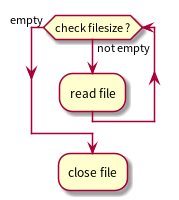
\includegraphics[width=.9\linewidth]{imgs/test.png}
\end{center}
\end{frame}
\begin{frame}[label={sec:org79997d7}]{Questions}
请 \alert{随时} 打断提问
\begin{columns}
\begin{column}{0.45\columnwidth}
\begin{block}{}
\begin{center}
\includegraphics[width=.9\linewidth]{imgs/avatar.png}
\end{center}
\end{block}
\end{column}
\begin{column}{0.45\columnwidth}
\begin{block}{}
\begin{center}
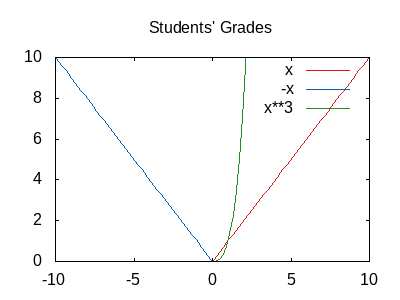
\includegraphics[width=.9\linewidth]{imgs/grades.png}
\end{center}
\end{block}
\end{column}
\end{columns}
\end{frame}
\section{XX algorithm}
\label{sec:orgd20dca1}
\begin{frame}[label={sec:orgeb8c952}]{Auto Exoposure}
\begin{itemize}
\item 测光方法
\begin{itemize}
\item Full
\item Center
\item histogram
\end{itemize}
\item Target calibration
\end{itemize}

\center\rule{0.5\paperwidth}{0.4pt}

\begin{itemize}
\item Control algorithm
\end{itemize}
\end{frame}
\begin{frame}[label={sec:org42bd769}]{Auto white balance}
\begin{block}{An unblanced image}
\framedgraphic[0.6]{imgs/test.png} \footnote{图片来自网络}
\end{block}
\end{frame}

\begin{frame}[label={sec:org63d3bad}]{Auto white balance}
\begin{block}{After balance}
\begin{columns}
\begin{column}{0.45\columnwidth}
\begin{block}{M-x describe-gnu-project}
\begin{itemize}
\item GCC
\item GNU
\item Emacs
\end{itemize}
\end{block}
\end{column}
\begin{column}{0.45\columnwidth}
\begin{block}{}
\begin{itemize}
\item GPL
\item FSF
\item GNU/Linux
\end{itemize}
\end{block}
\end{column}
\end{columns}
\begin{block}{Over}
\end{block}
\end{block}
\end{frame}
\begin{frame}[label={sec:org6e0b067},fragile]{Auto white balance}
 \begin{block}{Code sample}
\begin{minted}[bgcolor=bg,frame=lines,linenos=,fontsize=\scriptsize]{c}
int main(int argc, char *argv[])
{
        int a, b;

        printf("test print %d, %d\n", a, b);

        return 0;
}

\end{minted}
\end{block}
\end{frame}
\section{Summerize}
\label{sec:orga5bca62}
\begin{frame}[label={sec:orgb1887df}]{The end!}
\begin{block}{Q \& A}
\end{block}
\begin{block}{\alert{中文}}
\end{block}
\end{frame}
\end{document}